%note: don't split this document up with include{...}

\section{VisualGraph}

\subsection{Klassendiagramm}

\begin{figure}[H]
\centering
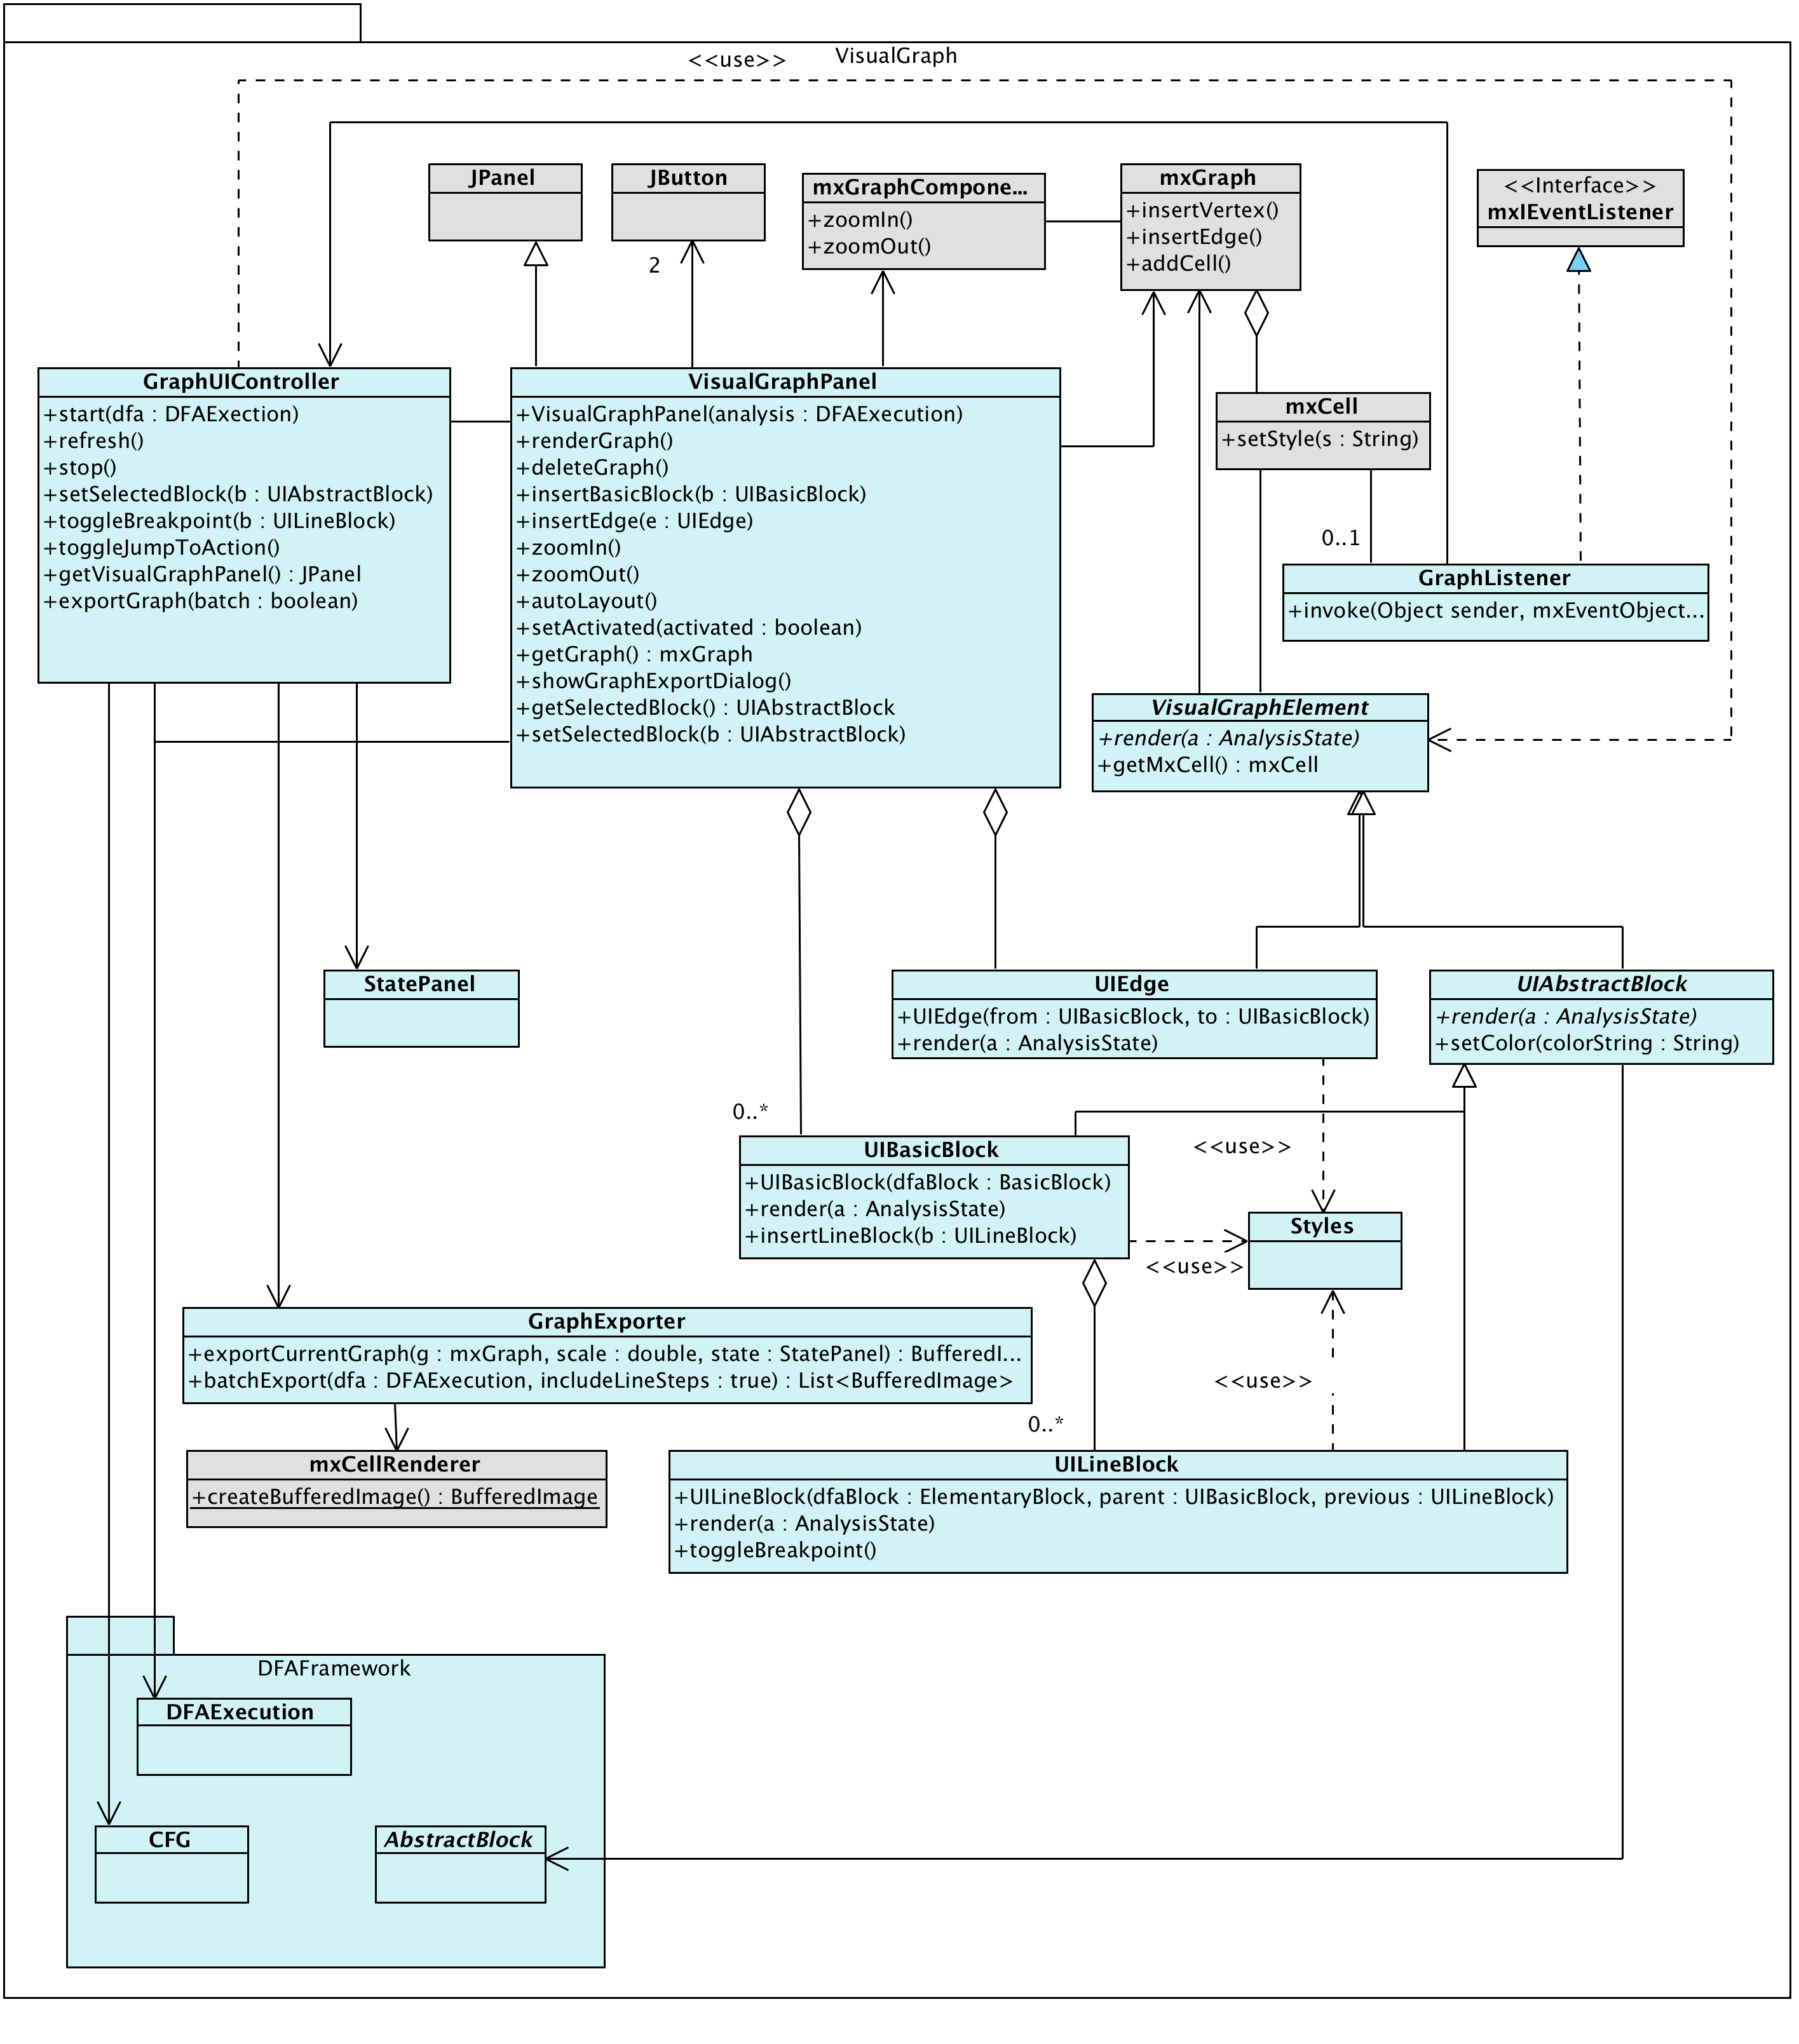
\includegraphics[width=1\textwidth]{Klassenuebersicht/VisualGraph/VisualGraph}
\end{figure}

\newpage

\subsection{Klassenbeschreibung}

Das VisualGraph-Modul ist dafür zuständig, aktuelle Daten aus dem DFAFramework abzufragen und diese visuell in einem Graphen darzustellen. 
Zusätzlich ermöglicht es dem Nutzer, Breakpoints für die Analyse zu setzen und den Graphen als PNG-Datei zu exportieren.

Als zentrale logische Schnittstelle bietet das VisualGraph-Modul die Klasse \inlinecode{GraphUIController}. 
Diese muss vom Controller-Modul über den Aufruf von start() oder refresh() darüber benachrichtigt werden, dass es Änderungen in der Analyse des DFAFrameworks gegeben hat.
Ist diese Benachrichtigung erfolgt, so beschafft sich der \inlinecode{GraphUIController} selbsttätig alle benötigten Daten vom DFAFramework, um die Objektstruktur für den visuellen Graphen zu erstellen und den Graphen zu rendern.

Die zweite nach außen wichtige Schnittstelle ist die Klasse \inlinecode{VisualGraphPanel}. Diese erbt von \inlinecode{JPanel} und beherbergt direkt den visuellen Graphen.
Zusätzlich stehen für die Visualisierung wichtige Methoden wie zoomIn(), zoomOut() und setActivated() zu Verfügung.
Die übrigen Methoden des \inlinecode{VisualGraphPanel}s werden ausschließlich von \inlinecode{GraphUIController}, \inlinecode{GraphExporter} und Listener-Objekten aufgerufen.

Bemerkenswert am Entwurf des VisualGraph-Moduls ist die Entkopplung der Visualisierungslogik von der benutzten Library JGraphX.
So arbeiten weder \inlinecode{VisualGraphPanel} noch \inlinecode{GraphUIController} direkt mit der Klasse \inlinecode{mxCell}, welche alle visuellen Komponenten in JGraphX repräsentiert.
Stattdessen wird auf eine eigene Struktur mit der Klasse \inlinecode{VisualGraphElement} und ihren Subklassen \inlinecode{UIEdge}, \inlinecode{UIAbstractBlock}, \inlinecode{UIBasicBlock} und \inlinecode{UILineBlock} gesetzt.
Jedes \inlinecode{VisualGraphElement} besitzt eine Referenz auf das \inlinecode{mxGraph}-Objekt, eine Referenz auf den zugehörigen logischen Block aus dem DFAFramework und eine render()-Methode.
Beim ersten Aufruf von render() wird nun dafür gesorgt, dass die entsprechende \inlinecode{mxCell} erstellt und in den \inlinecode{mxGraph} eingefügt wird.
Wird render() erneut auf dem selben Objekt aufgerufen, so aktualisiert es seine Daten, indem es diese beim DFAFramework abfragt.
Anschließend aktualisiert es seine zugehörige \inlinecode{mxCell}, um den angezeigten Graphen neu zu rendern.

Für den Entwurf ergeben sich folgende Vorteile:
\begin{itemize}
	\item Die Klassen \inlinecode{GraphUIController} und \inlinecode{VisualGraphPanel} müssen sich nicht mit Layouts, Größen oder Koordinaten auseinandersetzen, da dies von den \inlinecode{VisualGraphElement}-Subklassen erledigt wird.
	    Die Erstellung eines visuellen Grundblocks mit JGraphX ist komplex (für jede Zeile eines Grundblocks wird eine eigene verschachtelte \inlinecode{mxCell} benötigt, und Zeilen müssen alle untereinander gerendert werden).
	    Durch die gegebene Entwurfsarchitektur wird diese Komplexität versteckt, sodass der visuelle Graph sehr einfach erstellt werden kann.
	\item Durch die Entkopplung wird ein Austausch von JGraphX stark erleichtert, da in diesem Fall hauptsächlich die Subklassen von \inlinecode{VisualGraphElement} geändert werden müssen.
        Das \inlinecode{VisualGraphPanel} hat zwar ebenfalls eine Referenz auf \inlinecode{mxGraph}, allerdings nur, um diesen in den \inlinecode{mxGraphComponent} einzufügen. 
        Auch die getGraph()-Methode im \inlinecode{VisualGraphPanel} ist nur für den Batch-Export notwendig.
        Abgesehen davon wäre es also ausreichend, die Subklassen von \inlinecode{VisualGraphElement} und wenige Zeilen im \inlinecode{VisualGraphPanel} zu ändern, um JGraphX gegen eine andere Library auszutauschen.
        
\end{itemize}

% the template for one class description

\class{VisualGraphPanel extends JPanel}

Das Panel, welches den visuellen Graphen sowie Jump-to-Action- und Graph-Export-Button enthält. 
Es besitzt außerdem Methoden, um Blöcke und Kanten einzufügen, den Graphen zu rendern und zu zoomen.

\subparagraph{Konstruktoren} % skip this if there are no constructors
\begin{itemize}
	\item \ctor{VisualGraphPanel}{analysis: DFAExecution}{public}{
		Erstellt ein neues \inlinecode{VisualGraphPanel}, welches auf der gegebenen \inlinecode{DFAExecution} operiert.
	}
\end{itemize}

\subparagraph{Methoden}  % skip this if there are no methods
\begin{itemize}
	\item \method{renderGraph}{void}{}{public}{
		Erstellt bzw. aktualisiert den visuellen \inlinecode{mxGraph}-Graphen und macht diesen sichtbar.
		Dies geschieht durch Aufruf von render() auf allen hinzugefügten \inlinecode{VisualGraphElement}s.
	}
	\item \method{deleteGraph}{void}{}{public}{
		Entfernt den \inlinecode{mxGraph}-Graphen aus dem Panel und löscht ihn.
	}
	\item \method{insertBasicBlock}{void}{b: UIBasicBlock}{public}{
		Fügt den gegebenen \inlinecode{UIBasicBlock} ein, sodass dieser beim nächsten Aufruf von renderGraph() angezeigt wird.
	}
	\item \method{insertEdge}{void}{e: UIEdge}{public}{
		Fügt die gegebene \inlinecode{UIEdge} ein, sodass diese beim nächsten Aufruf von renderGraph() angezeigt wird.
	}
	\item \method{zoomIn}{void}{}{public}{
		Zoomt in den Graphen hinein durch Aufruf von \inlinecode{mxGraphComponent}.zoomIn().
	}
	\item \method{methodName}{void}{}{public}{
		Zoomt aus dem Graphen heraus durch Aufruf von \inlinecode{mxGraphComponent}.zoomOut().
	}
	\item \method{autoLayout}{void}{}{public}{
		Führt den Auto-Layouter auf dem angezeigten Graphen aus.
	}
	\item \method{setActivated}{void}{isActivated: boolean}{public}{
		Legt fest, ob das VisualGraphPanel Benutzerinteraktion ermöglichen soll.
	}
	\item \method{getGraph}{mxGraph}{}{public}{
        Gibt den \inlinecode{mxGraph} zurück. Diese Methode wird für den Graph-Export benötigt.
	}
	\item \method{setCurrentBlock}{void}{b: UIAbstractBlock}{public}{
		Setzt den aktuellen Block der Analyse. 
		Diese Methode wird beim Aufruf von render() eines \inlinecode{UIAbstractBlock}s aufgerufen, falls der entsprechende Block des DFAFrameworks gerade der aktuelle Block der Analyse ist.
		So wird gewährleistet, dass das \inlinecode{VisualGraphPanel} den aktuellen \inlinecode{UIAbstractBlock} kennt und die Jump-to-Action-Funktion benutzt werden kann.
	}
	\newpage
	\item \method{getSelectedBlock}{void}{}{UIAbstractBlock}{
		Gibt den \inlinecode{UIAbstractBlock}, der dem aktuellen Block aus der Analyse des DFAFrameworks entspricht, zurück.
		Diese Methode wird für die Jump-to-Action-Funktion benötigt und vom \inlinecode{GraphUIController} aufgerufen.
	}
	\item \method{showGraphExportDialog}{void}{}{public}{
		Zeigt den Graph-Export-Dialog an.
	}
\end{itemize}

\class{GraphUIController}
Der \inlinecode{GraphUIController} ist dafür zuständig, das \inlinecode{VisualGraphPanel} zu erstellen und die \inlinecode{VisualGraphElement}s darin einzufügen. 
Dazu bietet er die zentralen Methoden start(), update() und stop().
Diese werden vom Controller-Modul aufgerufen, sobald sich eine Änderung der Analyse des DFAFrameworks ergeben hat.

\subparagraph{Konstruktoren} % skip this if there are no constructors
\begin{itemize}
	\item \ctor{GraphUIController}{}{public}{
	    Erstellt einen neuen \inlinecode{GraphUIController} und ein zugehöriges \inlinecode{VisualGraphPanel}.
	}
\end{itemize}

\subparagraph{Methoden}  % skip this if there are no methods
\begin{itemize}
	\item \method{start}{void}{dfa: DFAExecution}{public}{
		Wird vom Controller nach Analysestart aufgerufen. 
		Durch diese Methode werden alle benötigten Daten vom DFAFramework abgerufen.
		Anschließend werden die \inlinecode{VisualGraphElement}s erstellt und in das \inlinecode{VisualGraphPanel} eingefügt.
		Danach wird renderGraph() auf dem \inlinecode{VisualGraphPanel} aufgerufen, um den Graphen anzuzeigen.
		Zuletzt wird autoLayout() auf dem \inlinecode{VisualGraphPanel} aufgerufen.
	}
	\item \method{refresh}{void}{}{public}{
		Wird vom Controller nach jedem Analyseschritt aufgerufen.
		Diese Methode ruft renderGraph() erneut auf, ohne autoLayout() auszuführen.
		Der angezeigte Graph wird dadurch aktualisiert. 
	}
	\item \method{stop}{void}{}{public}{
		Entfernt und löscht den angezeigten Graphen durch Aufruf von deleteGraph() auf dem \inlinecode{VisualGraphPanel}.
	}
	\item \method{setSelectedBlock}{void}{b: UIAbstractBlock}{public}{
		Setzt den aktuell ausgewählten Block durch Aufruf von setSelected() auf dem entsprechenden \inlinecode{UIAbstractBlock}.
	}
	\item \method{toggleBreakpoint}{void}{b: UILineBlock}{public}{
		Setzt bzw. entfernt einen Breakpoint durch Aufruf von toggleBreakpoint() auf dem entsprechenden \inlinecode{UILineBlock}.
	}
	\item \method{toggleJumpToAction}{void}{}{public}{
		Aktiviert bzw. deaktiviert die Jump-to-Action-Funktion. 
		Falls diese aktiviert ist, wird bei jedem Aufruf von refresh() der ausgewählte Block auf den aktuellen Block der Analyse gesetzt (durch Aufruf von setSelectedBlock())
	}
	\item \method{getVisualGraphPanel}{VisualGraphPanel}{}{public}{
		Gibt das \inlinecode{VisualGraphPanel} zurück.
		Diese Methode wird benötigt, um das Panel in das \inlinecode{ProgramFrame} einfügen zu können.
	}
	\item \method{exportGraph}{void}{batch: boolean}{public}{
		Erstellt einen neuen \inlinecode{GraphExporter} und führt den Export durch Aufruf von exportCurrentGraph() bzw. batchExport() auf dem \inlinecode{GraphExporter} durch.
	}
\end{itemize}

% the template for one class description

\class{abstract VisualGraphElement}
%Brief descrition of SomeClass.

\subparagraph{Methoden}  % skip this if there are no methods
\begin{itemize}
	\item \method{render}{void}{a: AnalysisState}{public abstract}{
		Erstellt eine (je nach Subklasse unterschiedliche) \inlinecode{mxCell} und fügt diese in das \inlinecode{mxGraph}-Objekt ein.
		Falls die \inlinecode{mxCell} bereits existiert, so wird diese mit den aktuellen Daten des entsprechenden Blocks des DFAFrameworks aktualisiert.
	}
	\item \method{getMxCell}{mxCell}{}{public}{
		Gibt die zugehörige mxCell zurück.
		Wird in der render()-Methoden des \inlinecode{UILineBlock}s und der \inlinecode{UIEdge} benötigt.
	}
\end{itemize}

\class{UIEdge extends VisualGraphElement}
Die Repräsentation einer Kante im visuellen Graphen.

\subparagraph{Konstruktoren} % skip this if there are no constructors
\begin{itemize}
	\item \ctor{UIEdge}{from: UIBasicBlock, to: UIBasicBlock}{public}{
		Erstellt eine neue \inlinecode{UIEdge} zwischen den entsprechenden \inlinecode{UIBasicBlock}s.
	}
\end{itemize}

\subparagraph{Methoden}  % skip this if there are no methods
\begin{itemize}
	\item \method{render}{void}{a: AnalysisState}{public}{
		Erstellt eine Kante im mxGraph-Objekt.
		Die im Konstruktor übergebenen \inlinecode{UIBasicBlock}s müssen bereits gerendert sein, damit die \inlinecode{UIEdge} erfolgreich gerendert werden kann.
	}
\end{itemize}

\class{abstract UIAbstractBlock extends VisualGraphElement}
Die Repräsentation eines Blockes (Parent- oder Zeilenblock) im visuellen Graphen.

\subparagraph{Methoden}  % skip this if there are no methods
\begin{itemize}
	\item \method{setSelected}{void}{isSelected: boolean}{public}{
		Bestimmt, ob die zugehörige \inlinecode{mxCell} ausgewählt sein soll.
	}
\end{itemize}

\newpage
\class{UIBasicBlock}
Die Repräsentation eines BasicBlocks im visuellen Graphen.

\subparagraph{Konstruktoren} % skip this if there are no constructors
\begin{itemize}
	\item \ctor{UIBasicBlock}{dfaBlock: BasicBlock}{public}{
		Erstellt einen neuen \inlinecode{UIBasicBlock}, welcher dem übergebenen \inlinecode{BasicBlock} entspricht.
	}
\end{itemize}

\subparagraph{Methoden}  % skip this if there are no methods
\begin{itemize}
	\item \method{render}{void}{a: AnalysisState}{public}{
		Erstellt einen Grundblock im \inlinecode{mxGraph}-Objekt und ruft render() auf allen zugehörigen \inlinecode{UILineBlock}s auf.
	}
	\item \method{insertLineBlock}{void}{b: UILineBlock}{public}{
		Fügt einen \inlinecode{UILineBlock} in den \inlinecode{UIBasicBlock} ein.
	}
\end{itemize}

\class{UILineBlock}
Die Repräsentation eines \inlinecode{ElementaryBlock}s im visuellen Graphen.

\subparagraph{Konstruktoren} % skip this if there are no constructors
\begin{itemize}
	\item \ctor{UILineBlock}{dfaBlock: ElementaryBlock, parent: UIBasicBlock, previous: UILineBlock}{public}{
		Erstellt einen neuen \inlinecode{UILineBlock}, der dem übergebenen \inlinecode{ElementaryBlock} entspricht.
	}
\end{itemize}

\subparagraph{Methoden}  % skip this if there are no methods
\begin{itemize}
	\item \method{render}{void}{a: AnalysisState}{public}{
		Erstellt eine Zeile in der Parent-\inlinecode{mxCell} und zeigt diese an.
	}
	\item \method{toggleBreakpoint}{void}{}{public}{
		Aktiviert bzw. deaktiviert die Anzeige eines Breakpoints in der Zeile.
	}
\end{itemize}

\class{GraphListener implements mxIEventListener}
Jede \inlinecode{mxCell} besitzt einen eigenen \inlinecode{GraphListener}, der Click-Events verarbeitet, um Methoden auf dem \inlinecode{GraphUIController} aufzurufen.

\subparagraph{Methoden}  % skip this if there are no methods
\begin{itemize}
	\item \method{invoke}{void}{sender: Object, evt: mxEventObject}{public}{
		Wird aufgerufen, wenn der Nutzer die zugehörige \inlinecode{mxCell} aufgerufen hat.
		Diese Methode ruft die dem Event entsprechende Methode des \inlinecode{GraphUIController}s auf.
	}
\end{itemize}

\class{Styles}

Diese Klasse besitzt Konstanten für die visuelle Anzeige des Graphen. 
Diese sind \inlinecode{mxGraph}-Style-Strings und Zahlenwerte, welche die Maße der Blöcke festlegen.

\class{GraphExporter}
Diese Klasse ist für den Graph-Export zuständig. Dies beinhaltet den Export des aktuellen Zustandes sowie den Batch-Export aller Zustände.

\subparagraph{Methoden}  % skip this if there are no methods
\begin{itemize}
	\item \method{exportCurrentGraph}{BufferedImage}{g: mxGraph, scale: double, state: StatePanel}{public}{
		Exportiert den aktuellen Graphen und eine Visualisierung des \inlinecode{StatePanel}s als Bild.
	}
	\item \method{batchExport}{BufferedImage}{dfa: DFAExecution, includeLineSteps: boolean}{public}{
		Führt einen Batch-Export aller Analyse-Zustände durch.
		Dabei wird mithilfe der übergebenen DFAExecution ein neuer \inlinecode{GraphUIController} und ein neues \inlinecode{VisualGraphPanel} mitsamt \inlinecode{mxGraph} erstellt.
		Dadurch wird die angezeigte Analyse durch den Batch-Export nicht beeinflusst.
		Mit den erstellten Objekten wird die Analyse dann vollständig durchgelaufen.
		Dabei wird nach jedem Schritt der Analyse der Graph mitsamt In- und Out-States durch Aufruf von exportCurrentGraph() als Bild exportiert.
	}
\end{itemize}
